\chapter{Apprentissage automatique pour le traitement de la parole}
"La tristesse de l'intelligence artificielle est qu'elle est sans artifice, donc sans intelligence." 1987 -
Jean Baudrillard

\section{Apprentissage automatique : définitions}

Dans le domaine de l'intelligence artificielle (IA), l'apprentissage automatique (machine learning, abrégé ML en anglais) regroupe des méthodes permettant à un système d'apprendre un comportement. Généralement, l'apprentissage automatique permet, à partir de données plus ou moins massives, d'apprendre à caractériser de nouvelles données de même nature par une classification ou une régression. On dit alors qu'un système automatique a été entraîné avec des données d’entraînement (première étape) afin de permettre la prédiction des caractéristiques de nouvelles données similaires (seconde étape).

\subsection{Classification et régression}
La classification et la régression sont les deux grandes familles d'apprentissage automatique.
La classification correspond à résoudre un problème d'affectation de classes. Par exemple, on peut apprendre à un système de détecter la présence d'hippopotame au sein d'une image. Nous avons alors deux réponses possibles : la présence ou l'absence de l'animal. Ces réponses se transforment donc en classes, qui seront prédites par un apprentissage automatique de type classification. Nous avons donc un nombre défini et connu de catégories, donc un espace discret, qui sera utilisé par le système pour catégoriser chacune des données.

La régression quant à elle ne permet pas de catégoriser les données en classe, elle les inscrit dans un espace continu. Par exemple, on peut apprendre à un système de prédire la valeur d'un stock en bourses à partir des valeurs des jours précédents. Les réponses sont donc des nombres qui peuvent être positifs ou négatifs et qui ont une précision infinie. Nous avons donc une échelle de valeur dans laquelle le système va inscrire sa prédiction.

\begin{figure}
  \centering
  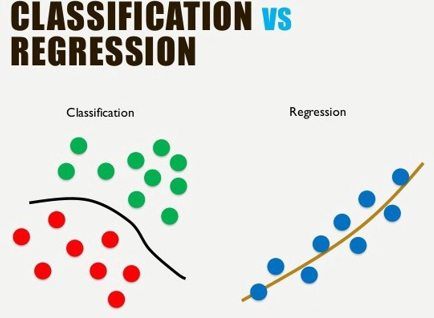
\includegraphics[width=8cm]{./Chapitre2/figures/classifVSreg.png}
  \caption{Représentation graphique de la classification et de la régression.}
  \label{fig:classifVSreg}
\end{figure}


Dans la figure~\ref{fig:classifVSreg}, on retrouve la différence graphique entre la classification et la régression. Pour une classification, le système automatique va chercher à mettre en place une démarcation entre les données de classes différentes, ici pour séparer les points verts et rouges. Tandis que pour une régression, le système va chercher la courbe qui minimise la somme des écarts de chaque point avec la courbe.

\subsection{Les facteurs de l'apprentissage automatique}
Un des facteurs les plus important pour la qualité de ces systèmes automatiques ce sont les données d’entraînement. Plus elles sont qualitatifs, c'est-à-dire qu'elles sont les pus proches des données réelles que nous voulons analyser, et plus le système sera performant dans sa tache de prédiction. Mais la qualité ne fait pas tout dans ce contexte, la quantité et l'exhaustivité sont tout aussi importantes.

Mais les données ne font pas tout, le choix de l'algorithme mis en place pour apprendre le système automatique est tout aussi important. Il existe de nombreuses méthodes mathématiques permettant de modéliser un système automatique. Ces derniers sont communément divisés en deux groupes, les méthodes d'apprentissage automatique et les méthodes de réseaux de neurones, appelé Deep Neural Network en anglais (DNN).
Le choix des données et du modèle est donc la principale question à se poser lorsque nous mettons en place des apprentissages automatiques.

Ces choix doivent être en adéquation avec le type de caractérisation recherché. En effet, il existe deux principaux types d'apprentissage : l'apprentissage supervisé et l'apprentissage non-supervisé.

\subsection{Apprentissage supervisé et non supervisé}

\begin{figure}
  \centering
  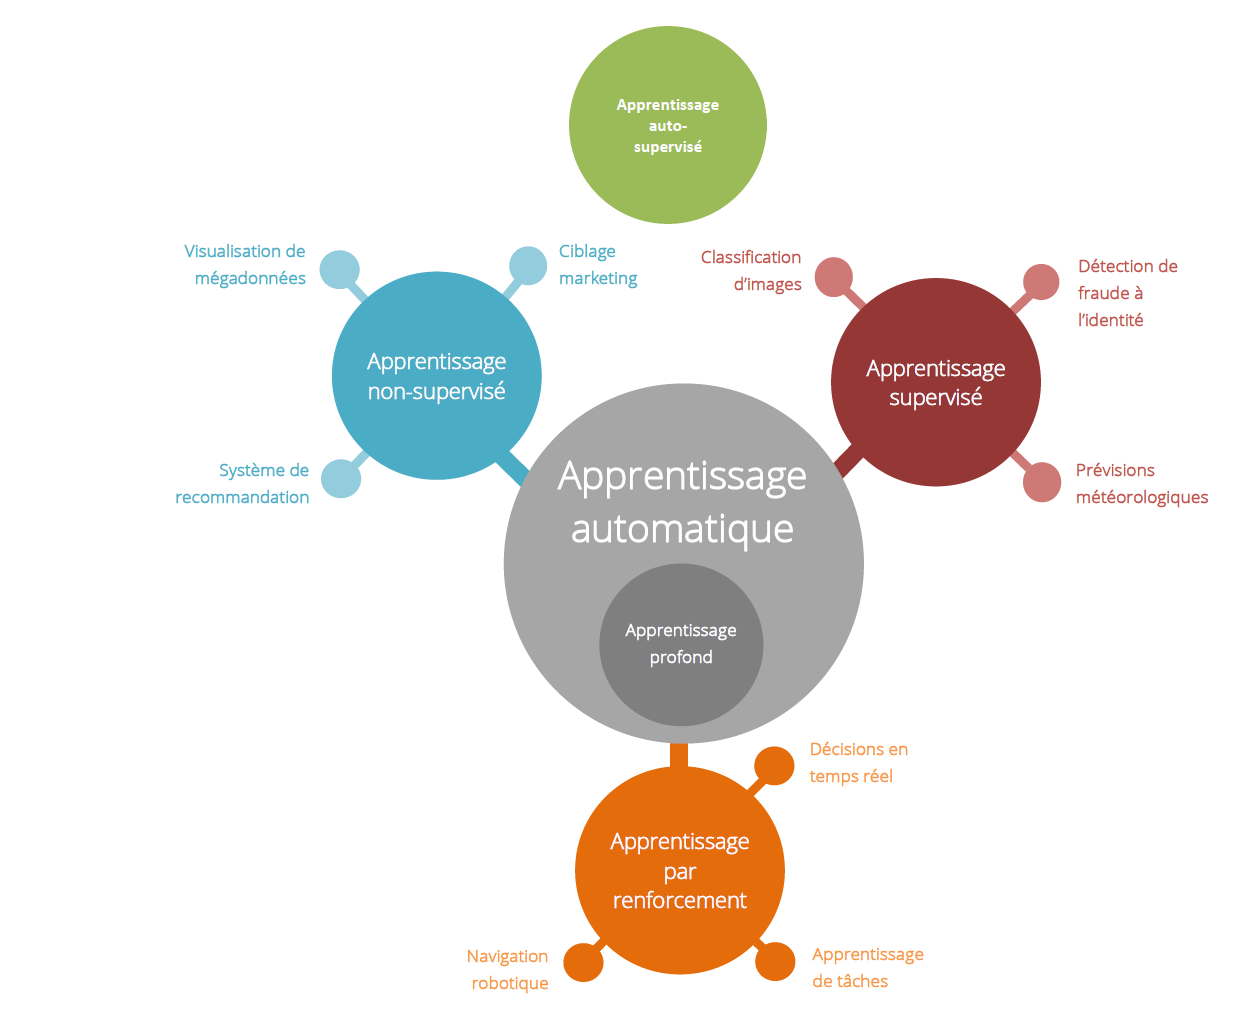
\includegraphics[width=.95\textwidth]{./Chapitre2/figures/typeApprentissage.png}
  \caption{Les différents types d'apprentissage et des exemples d'utilisation.}
  \label{fig:typeApprentissage}
\end{figure}

Il existe de nombreux type d'apprentissage dont les principaux sont présentés dans la figure~\ref{fig:typesApprentissage}. Dans le contexte de cette thèse, nous ne parlerons que d'apprentissage supervisé, non supervisé et auto-supervisé.

Lorsque nous parlons d'apprentissage supervisé, nous connaissons déjà les sorties souhaitées pour nos données d’entraînement. Nous avons une référence pour chaque document contenu dans les données d’entraînement et nous apprenons au système à retrouver ces références.
Il y a plusieurs mots pour définir ces références, on peut parler d'étiquettes, d'annotation ou de label. Ce type d'apprentissage ne peut donc être mis en place que lorsque nous avons des données d’entraînement qui sont annotées soit par l'humain soit automatiquement par un autre système d'apprentissage ou par un ensemble de règle par exemple. L'apprentissage supervisé peut être soit une classification, soit une régression.

Tandis que pour l'apprentissage non supervisé, nous ne connaissons pas les sorties attendues pour nos données d’entraînement. L'objectif du système automatique est donc de proposer une caractérisation des données d'entrée, en se basant sur des comparaisons entre ces dernières. Par exemple, on peut détecter la présence d'un hippopotame dans des images sans pour autant avoir des données annotées. Nous spécifions le nombre de classe au système et il va essayer d'apprendre tout seul ce qui différencie les images en entrée, ici la présence ou l'absence de l'animal. L'apprentissage non supervisé peut également servir à prédire une régression.

Un nouveau type d'apprentissage est de plus en plus utilisé, notamment dans le domaine de traitement des langages naturels (TALN), c'est l'apprentissage auto-supervisé, self supervised learning en anglais (SSL). Il s'agit d'un apprentissage où l'on n'a pas d'étiquette pour nos données d'apprentissage. Pour compenser leur absence, on prend une très grande masse de données et on en cache une partie. Le système devra alors retrouver les parties cachées à partir des parties disponible. Ainsi le système crée à la volée des étiquettes qui lui permettront d'apprendre.
Cette technique est utilisé par exemple dans la traduction de texte, où l'on apprend à représenter deux langues différentes puis en comparant ces deux représentations, on est capable de passer d'une langue A à une langue B sans avoir fourni au système des traductions d'un document de la langue A vers la langue B.

\textcolor{red}{est ce que je détaille l'apprentissage par renforcement?}

\section{Quelques familles d'apprentissage automatique}
Dans le contexte de la reconnaissance d'émotion, de nombreuses méthodes d'apprentissage automatique sont utilisées, que ce soit pour faire de la classification lorsque l'on considère une émotion comme discrète ou de la régression quand on considère une émotion comme continue.
Le tableau~\ref{tab:algoClassReg} met en évidence quels algorithmes utiliser en fonction de la tâche à accomplir. Dans les sections suivantes, nous détaillerons certaines d'entre elles.

\subsection{K moyen et K plus proche voisin}
Le k-moyennes, appelé k-means en anglais, et le k plus proche voisin, appelé k-nearest neighbors (KNN) sont des algorithmes de classification très simples. Ils sont principalement utilisés pour de la classification.
Le k-moyennes permet de diviser les données en k groupes distincts, appelés clusters. Le nombre de classe k est fixé par l'humain. Nous sommes donc dans un contexte d'apprentissage non supervisé.
Les k premières données sont définies comme les références des k classes puis on considère la distance entre les nouvelles données et ces références pour leur affecter une classe. La fonction à minimiser est donc la somme des carrées de ces distances.

Le k plus proche voisin est, quant à lui, un algorithme utilisé en classification supervisé. Le nombre de classe k est donc connu et on cherche à caractériser des données en fonction de leur distance avec les données contenues dans les k classes. On décide donc de la classe d'une donnée en fonction de ces plus proches voisins.

Ces deux algorithmes est donc très dépendants de l'initialisation du système : le nombre de classe ainsi que l'ordre de visualisation des données dans l'apprentissage sont des paramètres critiques.


\subsection{Classification naïve bayésienne}
La classification naïve bayésienne se base sur le théorème de Bayes. Ce théorème, qui se traduit par l'équation~\ref{eq:bayes} permet de prédire la probabilité conditionnelle de l'évènement A sachant B ($P(A|B)$) à partir des probabilités de l'évènement A ($P(A)$), l'évènement B ($P(B)$) et la probabilité de l'évènement B sachant A ($P(B|A)$).
\begin{equation}
    P(A|B) = \dfrac{P(B|A)*P(A)}{P(B)}
    \label{eq:bayes}
\end{equation}

Il prend chacune des caractéristiques des données indépendamment pour faire sa classification : il suppose une indépendance entre les différentes caractéristiques, d'où son appellation de \textit{naïf}. Par exemple pour la présence d'hippopotame dans un zoo, la présence d'un bassin et le nombre d'animaux ne seront pas pris en compte conjointement.

Son plus grand avantage c'est qu'il nécessite relativement peu de données d'entraînement pour estimer les paramètres nécessaires à la classification, à savoir moyennes et variances des différentes caractéristiques. Grâce au principe d'indépendance des caractéristiques, on n'a pas besoin de calculer la covariance entre ces dernières, ce qui permet au classifieur d'être rapide à apprendre et de ne pas nécessité des grandes puissances de calcul.

\subsection{Régression Linéaire}
La régression linéaire permet de catégoriser des sous-espaces en fonction de la proximité des données. Elle est à l'origine mise en place pour des régressions mais peut également être utilisée pour des classifications. Nous allons apprendre  pour chaque classe une fonction de régression linéaire qui est la plus optimale pour représenter les données de la classe. La régression linéaire peut être simple, représentée par une fonction affine $a*x+b$, pour des données mettant en lien deux variables, par exemple prédire la présence d'un hippopotame dans un zoo. Elle peut également être multiple, représentée par une fonction de type $a_1*x_1 + a_2*x_2 +... + b$  lorsque plusieurs données sont prises en compte, par exemple pour prédire la présence d'un hippopotame dans un zoo, nos données représentent la présence d'un zoo dans une ville, le nombre d'animaux qui le compose, la présence d'un bassin,...

Afin de classifier une nouvelle donnée, le système va comparer cette données avec les différentes courbes de régression utilisées pour modéliser les données en calculant l'écart de cette donnée à la courbe. On appelle cette méthode, l'estimateur des moindres carrés.
\textcolor{red}{besoin d'expliciter la méthode des moindres carrés?}
Cette méthode est simple, explicable et facile à mettre en place. L'apprentissage est également très rapide. Mais elle ne fonctionne pas pour toutes les tâches et toutes les données. En effet, elle implique que les données ont toutes une forte corrélation entre elles, ce qui n'est pas forcément le cas.

\subsection{Machine à vecteurs de support}
Cette méthode, appelée Support Vecteur Machine (SVM) en anglais, est utilisée pour résoudre des tâches de classification principalement et dans une moindre mesure de régression de façon supervisée. Elle consiste en la séparation linéaire des données projetées dans un espace en utilisant un hyperplan optimal. Cette séparation va être effectuée en maximisant la marge entre les données de chaque classe : l'hyperplan optimal doit être le plus éloigné des données des classes tout en les séparant.

Afin de classifier une nouvelle donnée, le système va donc placer cette donnée dans l'espace de représentation et situer son emplacement par l'hyperplan séparateur.
Cette méthode est très utilisée en classification, étant simple à mettre en place et rapide à apprendre. De plus, elle est très performante lorsque l'on possède peu de données d'apprentissage.

\subsection{Modèle de Markov cachés et modèle de mélange gaussien}

Le modèle de Markov caché, appelé hidden Markov model (HMM) en anglais, est un modèle statistique à base d'automates. Ces automates se composent d'états qui sont reliés par des transitions. Chaque transition va vers l'avant et correspond à la probabilité de changer de l'état courant pour le suivant. Comme le changement d'état n'est pas obligatoire, une transition circulaire est mise en place pour boucler sur l'état courant.
Utilisée en classification principalement, en apprentissage supervisé ou non, il va considérer chaque caractéristique d'une donnée une par une pour prédire son état final.

Le modèle de mélange gaussien, appelé Gaussien Mixture Model (GMM) en anglais, est très souvent associé aux HMM. En effet, il permet d'associer un ensemble de densités de probabilité aux les états, selon une loi gaussienne. Les paramètres de ces dernières sont apprises lors de la phase d'apprentissage par la maximisation de la vraisemblance. Le nombre de gaussienne est donné par l'humain.

Les modèles de Markov cachés sont massivement utilisés notamment en reconnaissance de formes, en intelligence artificielle ou encore en traitement automatique du langage naturel. Couplée aux GMM, ils ont longtemps été les systèmes à l'état de l'art pour la reconnaissance de la parole.
\textcolor{red}{besoin de plus d'explication? Figure, équation ou exemple concret ?}

\subsection{Réseau de neurones}
Les réseaux de neurones ont été conçus en s'inspirant du fonctionnement du cerveau humain. Ils sont donc composés d'une succession de neurones qui sont interconnectés entre eux pouvant ainsi propager des signaux.
Afin de mieux comprendre leur fonctionnement, il est intéressant de les mettre en relation avec la biologie du système nerveux de l'humain.
Au début du XXe siècle, les avancées de la biologie ont permis de mettre en lumière les méthodes de fonctionnement de notre système nerveux. On définit alors les neurones en tant que corps cellulaire muni d’un axone et de dendrites. Cette cellule, décrite dans la figure~\ref{fig:neuroneBio} est traversée par des influx nerveux de type électrique, qui entre par les dendrites et ressort par les synapses de son axone. Chaque neurone peut être reliés par un ou plusieurs neurones, que ce soit en entrée ou en sortie.
C'est en 1943 que Warren Sturgis McCulloch et Walter Pitts proposent une représentation mathématique des neurones, qu'on appelle neurone logique dans la suite de ce document. Ils définissent plusieurs principes :
\begin{itemize}
  \item un neurone biologique peut être représenté par un neurone logique,
  \item les entrées du neurone logique sont comparables aux dendrites,
  \item le neurone logique possède une seule sortie qui représente l'axone,
  \item les connexions entre les neurones se font par le clonage de la sortie en autant de liens qu'il y a de prochaines neurones, ce qui représente les connexions synaptiques,
  \item la fonction d'activation correspond à une prise de décision au niveau du neurone logique qui représente un potentiel d'activation : le neurone biologique ressort un influx nerveux ou pas.
\end{itemize}
C'est à partir de ces règles que les réseaux de neurones profonds, appelé deep neural network (DNN) vont être définis, afin de miner le processus d'apprentissage chez les humains.

\section{Réseau de neurones profonds}
Les réseaux de neurones profonds sont aujourd'hui très à la mode. Pourtant, ils ne sont pas récents : le premier algorithme d'apprentissage utilisant un réseau de neurone date de 1957 où Franck Rosenblatt propose le perceptron.

\subsection{Du perception au multicouche}
Le perceptron, schématisé dans la figure~\ref{fig:perceptron}, est un modèle qui permet de classifier les données en deux classes. Il s'agit donc d'un modèle qui permet de faire de la classification et de la régression de manière supervisée. Ce modèle binaire utilise un neurone pour l'apprentissage et la prédiction de la classe de chaque document. Un document est défini par x caractéristiques, chacune d'entre elles étant considérés comme une entrée du perceptron. Lors de l'apprentissage, des poids, initialisés de façon aléatoires, sont mis à jour pour chacune des entrées en fonction du taux d'apprentissage, appelé learning rate en anglais, afin de retrouver les étiquettes déjà connues des données d'apprentissage. En plus du poids, le biais est également défini lors de l'apprentissage. Le biais correspond à un unique poids qui sera utilisé pour la prédiction des étiquettes des données. Les entrées sont ainsi agrégées en les pondérant selon leur poids. La fonction d'agrégation est explicité par l'équation~\ref{eq:aggregation}, où $i$ correspond à l'entrée i, $w_i$ correspond au poids associé à l'entrée i et $\theta$ correspond au biais.
\begin{equation}
  z = \sum_{i=1}^{n}(w_i*i) - \theta
\end{equation}
Une fonction d'activation est ensuite appliquée : selon la valeur de $z$, la fonction donne un résultat de 0 si elle n'est pas activée ou de 1 si elle est activée. Dans le cas du perceptron de Rosenblatt, soit le tout premier perceptron, la fonction d'activation est définie par une fonction non linéaire qui prend une valeur de 0 si $z$ est inférieur ou égal à 0 et une valeur de 1 s'il est strictement supérieur à 0.
Il existe d'autres fonctions d'activation qui peuvent être utilisées, elles sont définie dans la section~\ref{sec:fonctionActivation}.

Le perceptron est une architecture très simple qui est de moins en moins utilisée. En effet, elle permet de résoudre uniquement des problèmes binaires linéairement séparables. Le perceptron multicouche est notamment capable de palier à ces inconvénients.

Le perceptron multicouche, appelé multilayer perceptron (MLP) en anglais, assemble plusieurs perceptrons entre eux comme illustré dans la figure~\ref{fig:perceptronMLP}. Un ou plusieurs neurones sont donc assemblées les uns à la suite des autres. Ils peuvent également formés des couches (layers) lorsqu'il y a plus d'un neurone qui traite les entrées. On a donc forcément une couche de neurones en entrée, donc qui prennent les données et une couche de neurones en sortie qui vont prendre la décision finale. Entre les deux, on peut retrouver des couches intermédiaires dites cachées, qui vont prendre en entrées les sorties de la couche précédente (soit la couche d'entrée, soit une autre couche cachée) et en sortie la couche suivante (soit une autre couche cachée soit la couche de sortie).
Les informations vont donc être propagées de gauche à droite, c'est-à-dire de la couche d'entrée à la couche de sortie. On appelle donc cette propagation, propagation directe avant, forward propagation en anglais. Le nombre de couche et le nombre de neurone par couche doit être défini par l'utilisateur pour être en adéquation avec la tache visée. Par exemple, le nombre de neurones de sortie permet de définir le nombre de classes dans une classification.
Si on se replace dans le contexte de l'apprentissage neuronal profond, le perceptron multicouche correspond à l'une des premières architectures dite profonde. En effet, elle est constituée d'au moins deux couches. Les chercheurs admettent que le nombre de couche est croissant en fonction de la difficulté de la tache à accomplir. Mais plus le système est complexe, donc plus il a de couches et de neurones par couche, plus il sera difficile de l'apprendre car il demandera beaucoup de données et de puissance de calcul.
En partant du principe de couches successives, de nombreuses architectures particulières ont vu le jour comme nous le définirons dans la section~\ref{sec:architecture}. Mais avant d'explorer les architectures, nous allons nous intéresser aux méthodes d'apprentissages.

\subsection{Algorithme d'apprentissage}
L'apprentissage des réseaux de neurones peut se résumer grossièrement en apprentissage de différents paramètres, dont des poids et des biais, qui permettent de prédire une référence, que ce soit une classe ou une valeur, à partir d'un ensemble de caractéristiques, appelés features en anglais, d'une données. Ces paramètres sont ajustés au fur et à mesure de la visualisation des données d'apprentissage, afin de trouver des paramètres optimaux qui permettent de maximiser les bonnes prédictions des données d'apprentissage en fonction de leurs caractéristiques. Il est donc essentiel de mettre en place cet apprentissage sur des données d'apprentissage cohérentes avec la tache visée.

Afin de réaliser cet apprentissage, il est nécessaire de définir la fonction de coût et le gradient.
La fonction de coût correspond à une fonction que l'apprentissage va chercher à minimiser ou à maximiser et qui correspond à une distance entre les valeurs prédites par le système et les valeurs attendues (les références). Le gradient correspond au vecteur regroupant toutes les dérivées partielles de la fonction de coût.

\subsubsection{Fonction de coût}
Il existe de nombreuses fonctions de coût qui permettent de calculer l'écart entre les valeurs prédites et les valeurs de références. Grâce à des méthodes mettant en jeu le gradient, le rôle de l'apprentissage automatique sera de minimiser l'écart entre ces deux valeurs, afin de se rapprocher le plus possible des valeurs de référence et donc d'avoir un système performant.
Par exemple l'erreur quadratique moyenne, appelée mean square error (MSE) en anglais, est une fonction de coût très utilisée qui a pour avantage d'être simple et rapide à calculer. Elle consiste à calculer la différence entre l'observation, notée $O$, et la prédiction, notée $p$, d'une donnée selon l'équation~\ref{eq:mse} :
\begin{equation}
  MSE = 1/n*\sum_{i=1}^{n}(O-p)^2
  \label{eq:mse}
\end{equation}
$n$ correspond aux nombres d'observation. Parmi les fonctions de coût les plus utilisées, on peut citer la Racine de l'erreur quadratique moyenne (RMSE), la Classification Temporelle Connexionniste (CTC) ou encore la somme des carrés des résidus (SCR). C'est donc cette fonction de coût que l'on va dériver pour récupérer la valeur du gradient, que l'on utilise pour apprendre un système automatique.

\subsubsection{Rétropropagation du gradient}

Lors de la phase d'apprentissage, le système va chercher à minimiser les erreurs de prédiction. Pour ce faire, nous allons chercher la meilleure configuration de poids possible. L'algorithme de rétropropagation du gradient (backpropagation en anglais) va nous permettre de calculer l'erreur pour chacun des neurones en partant de la dernière couche et en remontant jusqu'à la première. Cette méthode, introduite par Rumelhart et al.~\cite{Rumelhart1986}, se divise en deux parties. Tout d'abord on calcule l'erreur globale en comparant les prédictions et les références, en utilisant la fonction de coût. Puis on va propager l'erreur de couche en couche, de la dernière jusqu'à la première.

Ainsi, la propagation des erreurs va permettre de modifier les poids associés à chaque neurone, en prenant en compte leur part dans l'erreur calculé. En fonction de la part de "responsabilité" d'un neurone dans l'erreur, son poids associé va être plus ou plus grandement modifié pour que le neurone deviennent plus activateur ou plus inhibiteur.
\textcolor{red}{besoin d'expliciter l'algo ?}

\subsubsection{Descente de gradient}
La descente du gradient est utilisée pour apprendre à minimiser la fonction de coût $C$. Comme nous l'avons défini plus tôt, le gradient correspond à un vecteur regroupant les dérivées partielles de la fonction de coût. Si on se place dans un système à une seule variable, le gradient correspond au coefficient directeur de la droite de régression linéaire. Comme il y a autant de dérivées partielles que de variables, le calcul de la valeur minimisant la fonction de coût demande trop de combinaison à tester. On utilise donc l'algorithme de descente de gradient qui revient à effectuer une approximation du minimum (ou du maximum dans certains cas) de la fonction de coût. \textcolor{red}{mal dit ?}
La méthode de descente en gradient consiste à mettre en place une variation des paramètres de la fonction de coût par des itérations successives. Ce pas est défini par le taux d'apprentissage (learning rate en anglais) noté $\alpha$. Ce taux permet de faire varier les paramètres de la fonction de cout lors des itérations. Pour chaque paramètres $x_1$, $x_2$, $x_n$ de la fonction de coût, la descente de gradient se définit par l'équation~\ref{eq:descente} :
\begin{equation}
  x_n+1 = x_n - \alpha*(\dfrac{dC(x)}{dx})
\end{equation}

Cet algorithme n'est pas exempt d'inconvénients. En effet, selon la fonction de coût considérée, il est possible qu'il existe plusieurs minimums mais qui ne correspondent pas au minimal global. On appelle ces zones des minima locaux : converger dans une de ces zones signifie une suboptimalité du réseau de neurones. En fonction du taux d'apprentissage utilisé, il est donc possible que l'algorithme de descente de gradient converge vers un minimum local à la place du minimum global. Plus le taux d'apprentissage est petit, plus il est possible de tomber dans cette configuration.

Cette descente de gradient connaît deux principales variantes : la descente de gradient stochastique et la descente de gradient par lot (batch en anglais). La descente de gradient stochastique va mettre a jour les paramètres après chacun des échantillon vu lors de l'apprentissage. La descente de gradient par lot va mettre à jour les paramètres après avoir vu tous les échantillons. La méthode de mini-batch correspond quant à elle à une méthode inspirée des deux variantes, la mise à jour des paramètres se fait après avoir vu un ensemble d'échantillon. Cette mise à jour est déterminée par l'équation~\ref{eq:SGD} où $W$ correspond aux poids, $\alpha$ au taux d'apprentissage et $C$ à la fonction de cout.
\begin{equation}
  w_{t+1} = w_{t} - \alpha\hat{\nabla}_{w}{C(w_{t})}
  \label{eq:SGD}
\end{equation}
Dans les systèmes de neurone actuels, cette troisième solution hybride est la plus utilisée puisqu'elle permet de diminuer le temps d'apprentissage tout en garantissant de bonnes performances.


\subsubsection{Algorithme d'optimisation du gradient}
Afin de rendre nos réseaux plus performants mais également à répondre à des problématiques de coût matériel et temporel, on utilise des algorithme d'optimisation du gradient. Ces algorithmes ont été développés dans un premier temps pour répondre à la problématique des minimaux locaux mais ils sont  aujourd'hui notamment utilisé pour diminuer le temps d'apprentissage sur des configurations matérielles limitées.
Les algorithmes d'optimisation adaptatifs que sont AdaGra et Adam sont les plus utilisés de nos jours. Ces derniers ont pour objectifs de changer dynamiquement les paramètres du système lors de l'apprentissage.

\subsubsubsection{AdaGrad}
AdaGrad, notation pour Adaptive gradient, a été introduit par Duchi et al.~\cite{Duchi2011}. Cette méthode d'optimisation de gradient permet d'adapter dynamiquement le taux d'apprentissage. La variation du taux d'apprentissage est proportionnelle à l'historique des mises à jour des paramètres du réseau de neurone. Ainsi, si un paramètre est peu fréquent, la mise à jour sera plus important et inversement. Ce nouvel taux d'apprentissage est défini à chaque époque par l'équation~\ref{eq:adagrad}.
\begin{equation}
  \theta_{t+1, i} = \theta_{t, i} - \frac{\alpha}{\sqrt{G_{t, ii} + \epsilon}}g_{t, i}
  \label{eq:adagrad}
\end{equation}
$\theta$ correspond au paramètre en cours de mise à jour, $\alpha$ au taux d'apprentissage. $G$ représente l'historique accumulé lors des précédentes époques. On ajoute un coefficient $\epsilon$ pour éviter la division par zéro, dans le cas où l'historique du gradient est égal à zéro. AdaGrad permet donc de faire évaluer le taux d'apprentissage automatiquement, rendant l'apprentissage plus efficace et robuste. Cependant l'algorithme tend à abaisser le taux d'apprentissage de façon drastique en fin d'apprentissage, ce qui stoppe l'apprentissage du système. Pour remédier à ce problème, une autre méthode est proposée.

\subsubsubsection{Rprop et RMSprop}
Rprop, introduit par Riedmiller et al.~\cite{Riedmiller1993} en 1993, est un algorithme d'optimisation de gradient par lot entier. Son objectif est de palier au problème des trop grandes variations du gradient. Quand des gradients sont très grands avec d'autres gradients très petits, il est alors compliqué de déterminer un taux d'apprentissage pertinent. De ce fait, cette méthode propose d'utiliser uniquement le signe des gradients. Ainsi on garantit une évolution de même ordre pour tous les poids. Cette évolution tend à éviter les plateaux et les minimums locaux, pour optimiser la convergence du système neuronal. Cet algorithme peut être diviser en trois étapes :
\begin{itemize}
  \item On considère le signe des deux derniers gradients et on les compare.
  \item S'ils sont du même signe et donc qu'ils vont dans la même direction, le prochain pas est multiplié par 1.2 pour aller plus vite dans la bonne direction. S'ils sont de signes contraires, alors notre ancien pas était trop important, on le diminue donc en multipliant par 0.5.
  \item On s'arrête quand on atteint une taille de pas défini par l'utilisateur en amont, en fonction des données.
\end{itemize}

Le problème de cet algorithme, c'est qu'il n'est pas performant pour une considération en mini-batch. RMSprop (Root Mean Square propagation), proposé par Hinton et al.~\cite{Hinton2013}, a pour objectif de palier à ce problème. Pour cela, on va conserver la moyenne glissante des carrés des gradients pour tous les poids. Ainsi on adapte le taux d'apprentissage avec la moyenne glissante et non avec la moyenne de chaque mini-batch. La moyenne glissante est calculée selon l'équation~\ref{eq:movingAVG} où $E[g^{2}]$ correspond à la moyenne glissante des gradients et $\gamma$ à une constante souvent fixée à 0.9.
\begin{equation}
  E\left[g^{2}\right]_{t} = \gamma E\left[g^{2}\right]_{t-1} + \left(1 - \gamma\right) g^{2}_{t}
  \label{eq:movingAVG}
\end{equation}
Une fois la moyenne glissante calculée, on peut définir le nouveau taux d'apprentissage selon l'équation~\ref{eq:RMSprop}, où on retrouve la moyenne glissante $E[g^{2}]$, le taux d'apprentissage $\alpha$ et $\epsilon$ une constante faible pour éviter la division par zéro.
\begin{equation}
  \theta_{t+1} = \theta_{t} - \frac{\alpha}{\sqrt{E\left[g^{2}\right]_{t} + \epsilon}}g_{t}
  \label{eq:RMSprop}
\end{equation}

Cet algorithme permet de remédier au problème d'AdaGrad. Mais un autre algorithme plus récent est aujourd'hui beaucoup plus utilisé.

\subsubsubsection{Adam}
L'algorithme Adam (Adaptative Moment Estimation), introduite par Kingma et al.~\cite{Kingma2015}, est l'une des méthodes les plus utilisées actuellement. Elle combine les avantages du Momentum et du RMSprop : elle corrige l'inconvénient de l'accumulation des gradients au carré et elle est appropriée pour les gradients bruités ou variant fortement. Le calcul des poids est réalisé selon l'équation~\ref{eq:Adam}. $w$ correspond aux poids, $\alpha$ au taux d'apprentissage, $m$ l'accumulation des gradients dont sa correction est défini par l'équation~\ref{eq:m} et $v$ l'accumulation des carrés des gradients dont sa correction est défini par l'équation~\ref{eq:v}. Les paramètres $\beta_{1}$ et $\beta_{2}$ correspondent à des taux de décroissance compris entre 0 et 1. Ils sont généralement fixés à respectivement 0.9 et 0.999. On utilise toujours un $\epsilon$ faible pour éviter une division par zéro. On utilise la correction de $m$ et $v$ pour palier au biais dénoté par les auteurs, lorsque les vecteurs sont proches de 0.
\begin{equation}
  w_{t} = w_{t-1} - \alpha\frac{\hat{m}_{t}}{\sqrt{\hat{v}_{t}} + \epsilon}
  \label{eq:Adam}
\end{equation}
\begin{equation}
  \hat{m}_{t} = \frac{\beta_{1}m_{t-1} + (1-\beta_{1})g_{t}}{1-\beta^{t}_{1}}
  \label{eq:m}
\end{equation}
\begin{equation}
  \hat{v}_{t} = \frac{\beta_{2}v_{t-1} + (1-\beta_{2})g_{t}^{2}}{1-\beta^{t}_{2}}
  \label{eq:v}
\end{equation}

Des variants de cet algorithme ont été publiés, dont AdaDelta~\cite{Zeiler2012} ou NAdam~\cite{Dozat2016} mais il reste l'algorithme majoritairement utilisé grâce à ces bonnes performances et la réduction apportée au temps d'apprentissage.

Les algorithmes d'optimisation du gradient ne sont pas les seuls leviers permettant une meilleure performance du système. En effet, tous ces algorithmes sont fortement impactés par l'initialiation des poids effectuée en début d'apprentissage.

\subsection{L'initialisation et ses enjeux}
Comme nous l'avons dit précédemment, l'initialisation des poids d'un modèle neuronal est très importante pour garantir de bonnes performances et une convergence rapide du système. Nous allons détailler dans cette section, quelques unes des techniques d'initialisation des poids utilisées de nos jour.


\subsubsection{Initialisation aléatoire}
La plus simple de ces initialisations est de déterminer des poids au hasard. Facile à mettre en place, elle ne favorise pas un apprentissage efficace. Cependant elle est toujours utilisée de nos jours pour sa rapidité d'exécution et sa performance toute relative. En fonction de l'aléatoire mis en place, elle peut conduire à des performances satisfaisantes voir optimales des réseaux de neurones. Cet aléatoire suit généralement des distributions définis par des lois statistiques tel que la loi normale ou la loi de poisson par exemple.

La méthode de Xavier, introduite par Glorot et al.~\cite{Glorot2010}, garde le principe de l'initialisation aléatoire tout en la contraignant. En effet, elle considère des poids aléatoires mais dont la moyenne des activation est égale à 0 et dont la variance doit être constante entre les couches neuronales.

En pratique, il faut effectuer plusieurs apprentissages avec des initialisations différentes, pour trouver plusieurs minima et retenir le système le plus performant. Cette stratégie permet également de quantifier l'impact de l'initialisation sur le système considéré. Il est néanmoins très difficile voir impossible de s'assurer que le minimum trouvé correspond au minimum global. En effet, Bishop et al. ont démontré que pour un systèmes à $n$ neurones, le nombre de minima locaux sont de $2^n*n!$.

Ils existent d'autres méthodes qui ne s'appuie pas sur une initialisation aléatoire, mais sur un apprentissage préalable de poids pour le réseau considéré.

\subsubsection{A partir de poids pré-appris}
La méthode de transfert d'apprentissage (transfert learning en anglais) est une méthode de plus en plus utilisée. Introduite par Pan et al.~\cite{Pan2009},elle propose que les poids des neurones soient appris en amont. Cet apprentissage se fait sur des données plus larges et ont pour but de mieux représenter les données utilisées, sur une tache proche de celle visée. Par exemple, pour effectuer de la reconnaissance d'entités nommées, on va dans un premier temps apprendre à reconnaître automatiquement la parole. Comme les entités nommées sont formées de mots, ces deux taches sont différentes mais proches. Ainsi, nous pouvons initialiser notre système avec des poids qui permettent de reconnaître des noms avant de reconnaître des entités nommées.

Comme nous avons effectué un apprentissage en amont, les poids des neurones ont pu se stabiliser une première fois. Les avantages de cette technique sont multiples. Dans un premier temps, elle permet d’accélérer la convergence d'un système. Comme nous avons déjà des poids stables et considérés comme assez proche de leur optimum, on se libère de toute une phase d'apprentissage pendant laquelle le système cherche une représentation correcte de ses données. Dans un second temps elle permet de palier au manque de données. Puisque les poids ont été initialisés sur d'autres données, proche de celle de la tache considérée, le pré-apprentissage peut être considérer comme une méthode d'augmentation de données.

Elle n'a pas que des avantages. En effet, il faut posséder d'autres données proche de celle de notre tache. Il faut également que la tache visée par le pré-apprentissage soit cohérent avec la tache courante. En temps qu'observateur humain, on peut définir deux taches comme étant proches alors que le réseau de neurone ne les considéra pas comme tel.

\subsubsection{Impact de l'initialisation}
Afin de quantifier facilement l'impact de l’initialisation, on peut utiliser un algorithme d'apprentissage simple : le k moyennes. Par définition, ce dernier est défini en fonction du nombre de classes k visée et de l'ordre de visualisation des données. Comme les k premières données sont considérés comme les premières données de chaque classe, il est assez intuitif de voir l'impact de cet ordre sur la classification finale des données. Un exemple est proposé sur la figure~\ref{fig:kmeans}. Deux classifications très différentes sont observées sur les mêmes données en fonction de l’initialisation du premier centroide.
\begin{figure}[ht]
  \centering
  \begin{subfigure}{.49\textwidth}
    \centering
    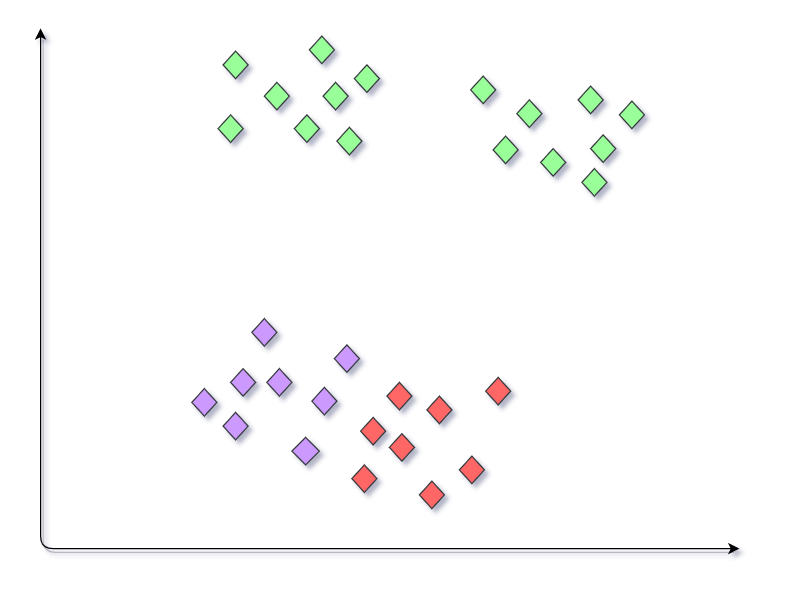
\includegraphics[width=.9\linewidth]{./Chapitre2/figures/kmeans1.png}
  \end{subfigure}
  \begin{subfigure}{.49\textwidth}
    \centering
    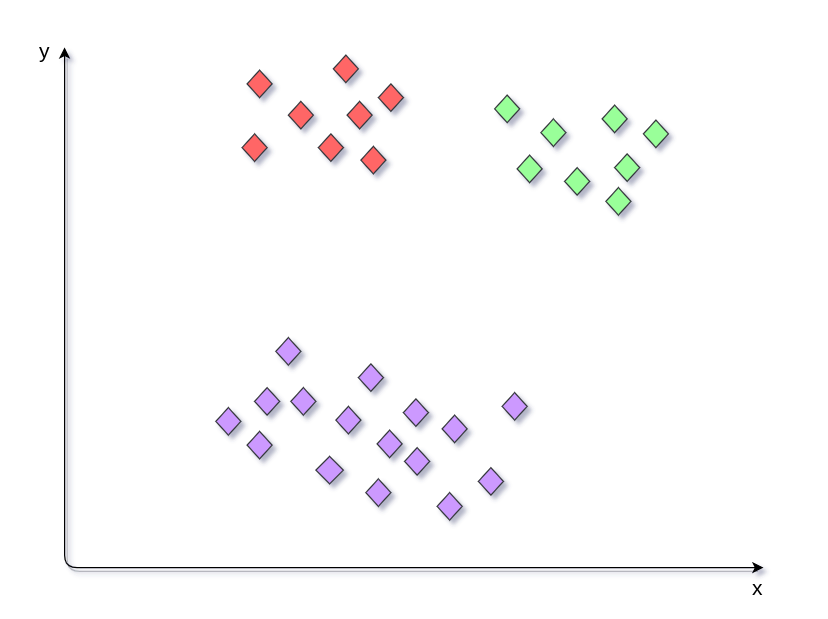
\includegraphics[width=.9\linewidth]{./Chapitre2/figures/kmeans2.png}
  \end{subfigure}
  \caption{Deux classifications en 3 classes utilisant l'algorithme k-moyennes avec deux initialisations de centroides différentes. Ici les données sont des points de coordonnées $(x,y)$. Illustrations issues de shorturl.at/htMN6 .}
  \label{fig:kmeans}
\end{figure}


Les réseaux de neurones sont eux aussi impactés par l'initialisation. En plus de dégrader les performances de la classification, une mauvaise initialisation peut allonger le temps d'apprentissage voir même empécher la convergence des systèmes. Il est donc important de considérer l’initialisation des systèmes comme un paramètre majeur de l'apprentissage automatique.

L’initialisation n'est pas le seul facteur à considérer lors d'un apprentissage automatique.

\subsection{La régularisation}
L’initialisation a son importance dans la performance d'un réseau de neurone, comme nous l'avons vu précédemment. Mais une bonne initialisation n'est pas suffisante pour garantir un système performant. Un des problèmes connu de l'apprentissage automatique est le sur-apprentissage. Ce problème peut être réglé par des méthodes dites de régularisation. Le sur-apprentissage et la régularisation sont définis dans cette section.

\subsubsection{Le sur-apprentissage}
Le sur-apprentissage, overfitting en anglais, est aussi appelé sur-ajustement. Il s'agit d'un phénomène naturel présent dans l'apprentissage lors duquel le système apprend à émettre les sorties exactes demandées pour les données d'apprentissage. Cela peut être rapproché de l'apprentissage par coeur chez les humains. En effet, lorsque le nombre de paramètres d'un réseau est trop important, et le nombre de données est faible, la minimisation de l'erreur de prédiction, définie par la fonction de cout, va conduire à un système parfaitement aligné aux données d’entraînement. On dit que ces systèmes sont très spécialisés et qu'ils ne sont pas capables de généraliser. En effet, lorsque nous lui présentons de nouvelles données, il ne pourra pas modéliser ces nouvelles informations et donnera des sorties proches de celles des données d’entraînement et non proches de celles des données réelles.

Ce phénomène est facilement identifiable : le score de la fonction de coût est très bon sur les données d’entraînement et très mauvais sur les données de développement et de test. Il suffit donc de vérifier l'écart entre les scores associées aux données d’entraînement et aux données de développement.  Si cet écart est trop prononcé et que le score sur les données d’entraînement est très bon, on peut en conclure que l'on se situe dans une configuration de sur-apprentissage.
\begin{figure}[ht]
  \centering
  \begin{subfigure}{.49\textwidth}
    \centering
    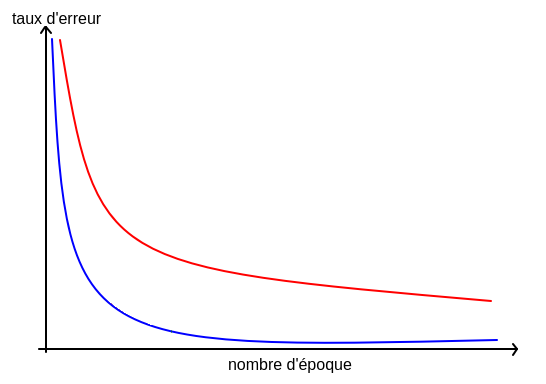
\includegraphics[width=.9\linewidth]{./Chapitre2/figures/surapprentissage2.png}
  \end{subfigure}
  \begin{subfigure}{.49\textwidth}
    \centering
    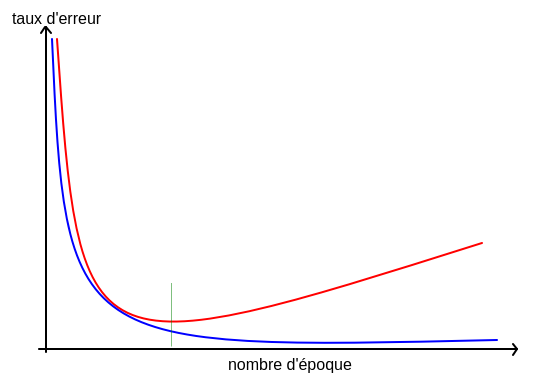
\includegraphics[width=.9\linewidth]{./Chapitre2/figures/surapprentissage1.png}
  \end{subfigure}
  \caption{Deux évolutions de scores sur les données d'entrainement en bleu et de développement en rouge. La figure de droite correspond à une situation de sur-apprentissage. Cette situation est observable à partir de l'époque correspondant à la ligne verte tracée.}
  \label{fig:surapprentissage}
\end{figure}


On peut voir sur la figure~\ref{fig:surapprentissage} l'évolution des scores constatés sur l'ensemble d'apprentissage et l'ensemble de développement. Dans la partie gauche, on constate une évolution normale des scores d'apprentissage sur l’entraînement (en bleu) et le développement (en rouge). Dans la partie droite, on remarque le sur-apprentissage qui correspond à la période où les deux courbes évoluent en sens contraires.

Plusieurs méthodes permettent de palier à ce phénomène. On a tout d'abord les méthodes passives, qui vont détecter les modèles en sur-apprentissage pour les supprimer. C'est ce que l'on met en place en utilisant un ensemble de développement ou de validation. On peut également diminuer le nombre de paramètres, en modifiant l'architecture neuronal ou augmenter le nombre de données d’entraînement. Il y a également les méthodes actives, qui sont également appelées méthodes de régularisation. Elles servent à contrôler la valeur des poids des neurones lors de l'apprentissage. La régularisation est la solution privilégiée pour prévenir ce problème comme Bartlett et al.~\cite{Bartlett1997} ont démontré que la valeur des poids était plus importante que le nombre de poids et donc de neurones pour éviter le sur-apprentissage. Il existe de nombreuses méthodes de régularisation. Nous allons considérer les régularisations les plus communes dans les prochains paragraphes.

\subsubsection{Régularisation L1 et L2}

La régularisation L1, ou Lasso Regression (Least Absolute Shrinkage andSelection Operator en anglais) a été introduite par Tibshirani~\cite{Tibshirani1996}. La régularisation L2 (Ridge Regression en anglais) quant à elle a été introduite par Hoerl et al.~\cite{Hoerl1970}. Ces deux régularisations mettent en place une pénalité qui est ajoutée à la fonction de coût. Elle diffèrent cependant sur la définition de cette pénalité. Utilisée pour pénaliser les poids les plus élevés, elles vont permettre la désactivation de certains neurones. La pénalité $p$ des régularisations L1 et L2 sont définies respectivement par l'équation~\ref{eq:L1} et~\ref{eq:L2}. $w$ correspond aux poids des neurones et $\lambda$ à un coefficient fixé par l'humain.

\begin{equation}
  p = \lambda\sum_{i=1}|w_i|
  \label{eq:L1}
\end{equation}

\begin{equation}
  p = \lambda\sum_{i=1}w^{2}
  \label{eq:L2}
\end{equation}

Comme on peut le remarquer, ces deux pénalités sont assez similaires. Soit on utilise la somme de la valeur absolue des poids, soit la somme des carrées des poids. Ces deux pénalités sont donc toujours positives.

\subsubsection{Normalisation des batchs}
Introduit par Ioffe et al.~\cite{Ioffe2015}, cette régularisation cherche à réduire les variations des données d'entrées de chacune des couches. Toutes les informations connues dans un réseau neuronal est inscrite dans un espace. L'objectif de l'apprentissage est de retrouver la meilleure représentation de ces informations de sorte que toutes les données d'une même classe soit dans le même espace. On appelle la différence entre les informations, le décalage des co-variables (covariate shift en anglais). Cet éloignement peut être observé entre toutes les représentations, qu'elles soient considérées de la même classe ou non. Cependant cet écart doit être réduit lors les données ont la même étiquette de sortie.

Une des façons de s'affranchir de ce problème est d'utiliser des lots, comme nous l'avons vu précédemment. Mais l'utilisation de batch ne va pas réduire la distance entre les représentations apprises par le système. Cette régularisation cible donc les représentations intermédiaires des données, à l'intérieur des couches cachées.

L'objectif de cette méthodes est de réduire le décalage des co-variables dans les couches cachées. Pour ce faire, on applique une normalisation à chaque entrée de neurones, quelque soit sa position dans les couches. Cette normalisation est définie par l'équation~\ref{eq:normbatch} où $\mu$ et $\sigma^2$ représente respectivement la moyenne et la variance du mini-lot $B$. $\epsilon$ est un coefficient faible ajouté pour éviter les division par zéro. Afin la valeur d'échelle $\gamma$ et la valeur de décalage $\bheta$ sont des paramètres qui sont appris pendant l'apprentissage.

\begin{equation}
  \hat{x}_{i}^{(k)} =\gamma ( \frac {x_i^{(k)}-\mu_B^{(k)}} \sqrt{\sigma_B^{(k)^2}+\epsilon} ) + \bheta
  \label{eq:normbatch}
\end{equation}

Cette normalisation permet d'éviter le sur-apprentissage. Elle permet également d'accélérer la mise en place de représentations internes cohérentes et donc de diminuer le temps d'apprentissage.

\subsubsection{Arret prématuré de l'apprentissage}
Une autre méthode largement utilisée consiste à arrêter l'apprentissage de façon précoce en fonction de la variation de l'erreur calculée à chaque époque (loss en anglais). En effet, si la variation de l'erreur est trop faible, il est très probable que l'on ait atteint un minimum local acceptable. Continuer l'apprentissage ne serait alors qu'une source de potentiel sur-ajustement. Cette méthode, appelée early stopping~\cite{Prechelt1996}, peut être appliquée sur la valeur de l'erreur sur les données d'apprentissage ou sur la valeur de l'erreur calculée sur les données de validation.

Bien que simpliste au premier abord, cette méthode est souvent utilisée car elle reste une normalisation très efficace~\cite{Finnoff1993} qui assure que le système ne sur-ajuste pas. De plus, il permet de réduire les temps d'apprentissage, puisqu'il diminue le nombre effectif d'époque.

\subsubsection{L'utilisation du dropout}
Le dropout, introduit par Srivastava et al.~\cite{Srivastava2014} est une normalisation très utilisée de nos jours. Elle consiste en la désactivation temporaire et aléatoire de neurones à chaque époque. Ainsi, le réseau a toujours des poids à apprendre et cela évite de tomber dans du sur-apprentissage. Comme le réseau est privé de certains de ces neurones, il doit apprendre à compenser cette perte, ce qui rend les représentations internes plus robustes et améliore la généralisation du modèle.

Ainsi, en fonction d'une probabilité $P$ de désactivation des neurones, souvent fixée à 0.5, le réseau aura plus ou moins de neurones désactivés et devra palier à ce manque de représentation.

Toutes ces méthodes permettent de garantir un fonctionnement correct voir optimal d'un système neuronal.

\section{Les architectures de couches neuronales utilisées dans le traitement de la parole}
Dans le cadre de cette thèse, nous travaillons sur les informations contenues dans la parole. Dans ce cadre, l'utilisation du MLP n'est pas la plus performante pour représenter les données de type parole. Il existe d'autres architectures de couches neuronales bien plus compatible avec ces données. En effet, le principe inconvénient du MLP, c'est qu'il n'y a pas d'influence des données précédentes et futures. Une entrée est donc considérée seule et sans contexte.

Hors nous savons que la parole est caractérisée par l'entièreté de sa séquence. Si nous faisons un parallèle avec un texte, une lettre seule ne veut rien dire. Accompagné d'autres lettres, elles forment un mot. Ces mots sont eux-mêmes agencés avec d'autres mots pour former un sens à une phrase.

Comme la parole est dépendante des états précédents, il est nécessaire d'utiliser des réseaux permettant de prendre en compte les états précédents voir les états suivants. Dans cette section, nous allons décrire des architectures neuronales permettant de conserver l'historique des états précédents, qui sont par conséquent utilisées dans le traitement de la parole.

\subsection{Réseau Convolutif}
Les réseaux neuronaux convolutifs (Convolutional Neural Network en anglais), abbrégé CNN~\cite{LeCun1990} sont prépondérant dans l'analyse d'image. En effet ils traitent des données représentées en deux dimensions comme des images (disposition des pixel en 2D). Ils sont également utilisés en parole, lorsque l'on considère le signal comme un spectrogramme.

Comme son nom l'indique, ce réseau effectue des produits de convolutions en fonction de la configuration de son champ recepteur. Il se décompose en trois opérations : la convolution, le pooling puis l'activation de type ReLu.
\subsection{RNN}
\subsection{LSTM et biLSTM}
\subsection{Encoder Decoder}
